\documentclass{beamer}
\usepackage{listings}
\lstset{
%language=C,
frame=single, 
breaklines=true,
columns=fullflexible
}
\usepackage{graphicx}
\usepackage{subcaption}
\usepackage{url}
\usepackage{tikz}
\usepackage{tkz-euclide}
\usetikzlibrary{calc,math}
\usepackage{float}
\newcommand\norm[1]{\left\lVert#1\right\rVert}
\renewcommand{\vec}[1]{\mathbf{#1}}
\usepackage[export]{adjustbox}
\usepackage[utf8]{inputenc}
\usepackage{amsmath}
\usetheme{Boadilla}
\title{Adaptive Congestion Control for mMTC in cellular network.}
\author{T. Rohan}
\institute{IIT H (CSE)}
\date{3rd May, 2021}
\begin{document}

\begin{frame}
\titlepage
\end{frame}

\begin{frame}
\frametitle{What is mMTC? What is the problem with it?}

$\bullet$ mMTC stands for Massive machine type communication.\\
$\bullet$ It is a type of communication between machines over wired or wireless networks where data generation, information exchange and actuation takes place with minimal or no intervention from humans.\\
$\bullet$ There is diverse traffic for different commands over various IoT applications, challenging the network efficiency.\\
$\bullet$ It suffers Congestion and signaling overload due to the high probability of collisions, especially in a dense network scenario.\\
$\bullet$ Now, we try to propose an adaptive grouping and strategy for the mMTC devices capable of reducing the number of simultaneous transmissions. Hence guarantee the successful transmission of the
data in the 5G cellular network. 

\end{frame}

\begin{frame}
\frametitle{mMTC RACH procedure in 5G network}
$\bullet$ 5G is the fifth generation of wireless communications technologies supporting cellular data networks.\\
$\bullet$The critical enhancements on the cellular network such as eMBB (enhanced Mobile Broadband), mMTC (massive Machine Type Communications), URLLC (Ultra-Reliable Low Latency Communications) characterize 5G.

\begin{enumerate}
\item State of the art of mMTC: The mMTC devices transmit small packet sizes of data following two traffic patterns:
    \begin{enumerate}
        \item Periodical : For applications such as Smart grid, periodical traffic pattern is used which is triggered as a Mobile Autonomous Reporting up-link transmission
        \item Event driven: For applications such as smoke alarm detectors, disaster alert, event driven traffic pattern is used, which is triggered by such emergency events.
    \end{enumerate}
\item RACH Procedure in 5G network :
        UE stands for User equipment, gNB for gNodeB.                       (contd. in the next slide)
\end{enumerate}


\end{frame}


\begin{frame}
\frametitle{RACH Procedure in 5G network}

 In the current Network scenario, UE performs the random access procedure as the initial contact between UE and the base station.\\
\begin{figure}[h]
\centering
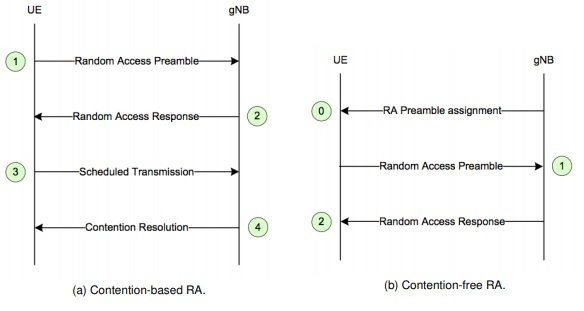
\includegraphics[width=0.6\textwidth]{Random access procedure.jpg}
\caption{5G Random Access Procedure.}
\label{fig:Figure 1}
\end{figure}
$\bullet$ As shown in figure \ref{fig:Figure 1}, there exists two types of random access procedure:
contention-based and contention-free. \\

\end{frame}


\begin{frame}
\frametitle{CBRA and CFRA}
\begin{block}{CBRA : Contention Based Random access}
$\bullet$ Also know as four step RACH Procedure. In this, UE selects a Preamble randomly from a pool of preambles shared with other UE, creating potential risks of selecting the same preamble as another UE and subsequently may experience conflict or contention.\\
$\bullet$The gNB uses a contention resolution mechanism to handle this, but, the result is random and not all Random Access succeeds.
\end{block}
\begin{block}{CFRA : Contention Free Random Access.}
$\bullet$ Also know as three step RACH procedure. In this, the Preamble is allocated by the gNB and such preambles are known as dedicated random access preamble. \\
$\bullet$The dedicated preamble is provided to UE either via RRC signalling or PHY Layer signalling, Thus, ensuring no preamble conflict.
\end{block}

\end{frame}



\begin{frame}
\frametitle{What is the problem ?}

$\bullet$ In the mMTC scenario,  to support a tremendous number of devices with zero/very low mobility transmitting occasionally in the network at a low bit rate, high density connection is needed.
\\
$\bullet$ Providing guaranteed network access to these devices presents a challenge for the network operators as the network will suffer for high MAC signaling overhead affecting the mMTC device’s energy efficiency characteristic.\\
$\bullet$ The high number of collisions in the contention-based random access procedure is surely leading to a failure of some mission-critical services.\\
$\bullet$ Hence the need for an efficient load control mechanism to
guarantee successful data transmission.

\end{frame}


\begin{frame}
\frametitle{Are there any existing approaches?}

$\bullet$ To streamline the messaging process.\\
$\bullet$ Sharing limited resources.\\
$\bullet$ forming device groups (one of the most effective techniques)\\
$\bullet$ some physical and medium access techniques\\ 

\end{frame}


\begin{frame}
\frametitle{Our approach}
$\bullet$ Our approach uses the application-to device relationship to enhance the grouping mechanism.\\
$\bullet$ It is done by transforming applications into task executions.\\
$\bullet$ Our algorithm performs the grouping on the task level. This reduces the signaling overload created as each member of the group.\\
$\bullet$ In other words, our grouping strategy will reduce the collision rate significantly.\\

\end{frame}



\begin{frame}
\frametitle{Problem Formulation.}
$\blacktriangleright$ When a set of mMTC devices need to access the network when triggered by some application, they will need to perform the tasks and report to the application server before the expiration time of the application.\\
$\bullet$ Any collision or delay during the RACH procedure side will affect the success probability of the data transmission.\\
$\blacktriangleright$ We aim to group the devices in such a way that all the tasks can be executed within the required time frame, preventing any failure. Hence the need to minimize the total number groups by optimally placing the right device in the group.\\
$\blacktriangleright$ This formulation is a variation of the 1D bin-packing problem and we use a modified version of the best-fit decreasing (BFD) algorithm to effectively group the MTC devices while respecting latency requirements.\\
\end{frame}


\begin{frame}
\frametitle{1D bin-packing problem}
The 1D bin packing problem could be simply put as:\\
$\bullet$ Given n items and n bins, with   
\begin{align}
w_j = \text{weight of the jth item}\\
c = \text{capacity of each bin.}
\end{align}
We have to assign each item to one bin so that the total weight of the items in each bin does
not exceed c and the number of bins used is a minimum. 

\end{frame}


\begin{frame}
\frametitle{Best Fit Decreasing Algorithm}
$\bullet$ First, we have to sort the items in decreasing order of their weights and assign them indices such that,
\begin{align}
w_1 \geq w_2 \geq \ldots \geq w_n
\end{align}
$\bullet$ Now, we assign the current item to the feasible bin (if any) having the smallest residual capacity (breaking ties in favour of the lowest indexed bin). If there exists no such bin which can accommodate a particular item, only then do we introduce a new bin.
\end{frame}


\begin{frame}
\frametitle {Analogy}
$\bullet$ The mMTC devices are analogues to the items in the 1D bin-packing problem.\\
$\bullet$ The groups which we make are analogues to the bins.\\
$\bullet$ Latency constraints of the applications represent bin sizes.

\end{frame}


\begin{frame}
\frametitle{Proposed Grouping Scheme}
$\blacktriangleright$ We integrate the scheduling mechanism by sorting in increasing order of the application’s time constraint. The grouping process starts by sorting devices in descending order
of their weight.\\
$\blacktriangleright$ For a device, the algorithm evaluates the device-dependent space of each group for all related applications. A device joins a group that has space to accommodate it with minimum remaining space.\\
$\bullet$ If there is no group with enough space to accommodate the device, a new group is created. It runs the iterations till all devices are grouped.\\
$\blacktriangleright$ Once grouped, the devices linked to a certain number of tasks in a group are then scheduled in the order of corresponding application’s expiration time, so that a task related to the most urgent application can be executed first.\\
$\bullet$ To prevent any frequent re-grouping, a relaxing factor $\gamma$ is introduced to control the extension of final bin sizes.The time constraint becomes $\gamma$ \times $\tau_m$ for further adjustment. The notion of miss rate is then added to the ratio of tasks executed after $\gamma$ \times $\tau_m$.


\end{frame}


\begin{frame}
\frametitle{Terms to know}
\begin{table}[h!]
  \begin{center}
    \begin{tabular}{|l|r|}
    \hline 
    Symbols & Meaning\\
    \hline
    \hline
    $T_i$ & Weighting time of ith device\\
    \hline
    $\tau_m$ & Applications' time constraint\\
    \hline
	$\gamma$ & Relaxing Factor\\
	\hline
	$\gamma$ \times $\tau_m$ & Total space of the bin\\
	\hline
	$\sum_j T_j$ \times $g_i.j$ & Total space occupied\\
	\hline
    \end{tabular}
  \end{center}
\label{Table:1}
\end{table}

\end{frame}

\begin{frame}
\frametitle{Algorithm 1}
\begin{figure}[h]
\centering
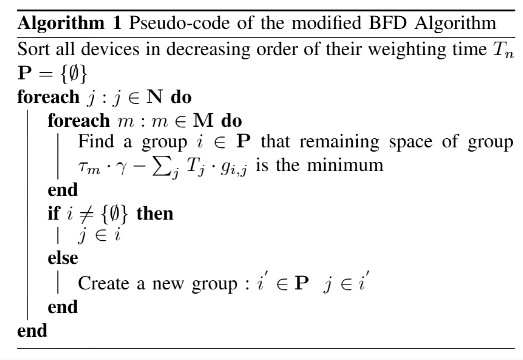
\includegraphics[width=0.8\textwidth]{Algorithm 1.png}
\caption{Algorithm 1.}
\label{fig:2}
\end{figure}
\end{frame}


\begin{frame}
\frametitle{Performance Analysis}
$\bullet$ Let there be 1000 to 5000 smart devices in the simulation setup.\\
$\bullet$ These devices collect, compute, record, and transfer resource consumption data, on demand, to the company responsible for applications such as monitoring and billing.\\
$\bullet$ The required number of groups and task missing rates are considered as the major performance indicator.\\
\end{frame}
\begin{frame}{Parameter Description and Values}
\begin{table}[h!]
  \begin{center}
    \begin{tabular}{||c|c|c||}
    \hline 
    Parameter &  Description & Value\\
    \hline
    \hline
    $N$ & No. of devices & 1000 to 5000\\
    \hline
    $K$ & No. of different tasks & 10 to 40\\
    \hline
	 & Tasks per application & 1 to 5, uniform distr.\\
	\hline
	 & Tasks per device & 1, 3, 5, uniform distr.\\
	\hline
	$M$ & No. of applications & 20\\
	\hline
	$t$ & Task time & uniform(0.1, 0.2)s\\
	\hline
	DpG(q) & Device per group with '$\gamma$ = q' & \\
	\hline
    \end{tabular}
  \end{center}
  \label{Table:2}
\end{table}

\end{frame}


\begin{frame}
\frametitle{Observations}
\begin{table}[h!]
  \begin{center}
    \begin{tabular}{||c|c|c|c|c|c|c||}
    \hline 
    Devices&DpG(0.3)&Miss&DpG(0.7)&Miss&DpG(1.1)&Miss\\
    \hline
    \hline
    1000 & 7.77 & 0 & 17.61 & 0.28 & 29.67 & 5.95\\
    \hline
    2000 & 7.14 & 0 & 18.35 & 0.01 & 27.04 & 6.00\\
    \hline
	3000 & 7.97 & 0 & 17.79 & 0.49 & 29.22 & 6.30\\
	\hline
	4000 & 7.57 & 0 & 18.03 & 0.54 & 28.11 & 5.89\\
	\hline
    5000 & 7.30 & 0 & 17.40 & 0.57 & 28.55 & 6.66\\
	\hline
    \end{tabular}
  \end{center}
  \label{Table:3}
  \caption{BFD performance with varying $\gamma$ in DpG, Tasks = 10}
\end{table}

\end{frame}


\begin{frame}
\frametitle{Observations}
$\bullet$ It is observed in the above table that when the packing factor $\gamma$ increases, the time constraint is relaxed and more devices can be assigned to the groups.\\
$\blacktriangleright$ But, more importantly, our modified BFD algorithm can support massive devices. The gap between the number of devices per group is small regardless of the number of devices (from 1000 devices to 5000).
\end{frame}


\begin{frame}
\frametitle{Conclusion}
$\blacktriangleright$ A grouping algorithm has been employed to deal with the congestion problem by finding the best grouping solution to minimize the number of simultaneous transmission in the context of mMTC devices in a 5G network. The obtained results clearly illustrate the grouping performance of our proposed algorithm and its impact on groups by lowering the miss rate probability in each group.
\end{frame}

\begin{frame}
\frametitle{Original Authors and Details}
$\bullet$ Boisguene Rubbens and Chih-Wei Huang
\\Department of Communication Engineering, National Central University, Taoyuan, Taiwan.\\
$\bullet$ 2020 IEEE International Conference on Consumer Electronics
- Taiwan (ICCE-Taiwan)
\end{frame}


\end{document}